\documentclass{article}
\usepackage[utf8]{inputenc}
\usepackage{amsmath}
\usepackage{amssymb}
\usepackage{amsfonts}
\usepackage{amsthm}
\usepackage{parskip}
\usepackage{bm}

\usepackage{pgfplots}
\pgfplotsset{compat = newest}

\newcommand{\N}{\mathbb{N}}
\newcommand{\Z}{\mathbb{Z}}
\newcommand{\Q}{\mathbb{Q}}
\newcommand{\R}{\mathbb{R}}
\newcommand{\C}{\mathbb{C}}

\renewcommand{\P}[1]{\mathbb{P}\left(#1\right)}
\newcommand{\E}[1]{\mathbb{E}\left[#1\right]}
\newcommand{\normal}{\mathcal{N}}
\newcommand{\var}[1]{\text{var}\left[#1\right]}
\newcommand{\gammafn}[1]{\Gamma\left(#1\right)}
\newcommand{\randsamp}{X_1,\dots,X_n}
\newcommand{\mgf}{moment generating function }
\newcommand{\pdf}{p.d.f. }
\newcommand{\pmf}{p.m.f. }
\newcommand{\cdf}{c.d.f. }
\newcommand{\clt}{central limit theorem}
\newcommand{\mle}{M.L.E. }
\DeclareMathOperator*{\Binomial}{Binomial}

\newenvironment{hwproof}[1]
{
    #1
    \begin{proof}
}{
    \end{proof}
}

\title{HW4}
\author{Asier Garcia Ruiz}

\begin{document}
\maketitle

\section{Section 8.1, problem 9.}
\begin{hwproof}
    {
        Let $\randsamp$ be a random sample form the exponential distribution with
        parameter $\theta$. Find the \cdf for the sampling distribution of the
        \mle of $\theta$. (The \mle itself was found in Exercise 7 in Sec. 7.5.)
    }

    We know that the \mle for the exponential distribution with parameter $\theta$
    is $\hat{\theta} = n / T$ where $T$ is the Gamma distribution with parameters
    $n$ and $\theta$. Let $G(\cdot)$ be the distribution of $T$, then we can write
    the \cdf of the sampling distribution $F(\cdot)$ as
    \begin{equation*}
        H(t) = \P{\hat{\theta} \leq t} = \P{\frac{n}{T} \leq t}
        = \P{T \geq \frac{n}{t} } = 1 - G\left(\frac{n}{t}\right).
    \end{equation*}
\end{hwproof}

\section{Section 8.2, problem 4.}
\begin{hwproof}
    {
        Suppose that a point $(X,Y)$ is to be chosen at random in the $xy$-plane,
        where $X$ and $Y$ are independent random variables and each has the standard
        normal distribution. If a circle is drawn in the $xy$-plane with its center
        at the origin, what is the radius of the smallest circle that can be chosen
        in order there to be a probability 0.99 that the point $(X,Y)$ will inside
        the circle.
    }
    From the general formula for a circle we know that
    \begin{equation*}
        X^2 + Y^2 = R^2.
    \end{equation*}
    We want to find $R$ such that any sample $(X=x, Y=y)$ are in the circle with
    probability 0.99. That is to say
    \begin{equation*}
        \P{x^2 + y^2 \leq R^2} = 0.99.
    \end{equation*}
    Now, since $X, Y \sim N(0,1)$ we know that $X^2, Y^2 \sim \chi^2(1)$.
    Furthermore, we know that $Z = X^2 + Y^2 \sim \chi^2(2)$. Using at the table
    from the back of the book we determine that $R^2 \geq 9.210$ and thus
    $R \geq \sqrt{9.210} = 3.035$.
\end{hwproof}
\section{Section 8.2, problem 7.}
\begin{hwproof}
    {
        Suppose that the random variables $\randsamp$ are independent,
        and each random variable $X_i$ has a continuos \cdf $F_i$. Also, let the
        random variable $Y$ be defined by the relation
        $Y = -2\sum_{i=1}^n \log F_i(X_i)$. Show that $Y$ has the $\chi^2$
        distribution with $2n$ degrees of freedom.
    }

    We know by the probability integral transformation (Thm 3.8.3) that each
    $Y_i = F_i(X_i)$ follows the uniform distribution on the interval $[0,1]$.
    Now, we let $Z_i = -\log{Y_i}$. We can calculate that since
    $Y_i = e^{-Z_i}$, $\frac{dt}{dz} = - e^{-Z_i}$. Thus, using a change of
    variable we find that the \pdf for $T_i$ is
    \begin{equation*}
        g(z) - f(e^{-z}) |\frac{dt}{dz}| = e^{-z}.
    \end{equation*}
    We observe that each $Z_i$ has the exponential distribution with parameter
    $\lambda = 1$, which is the same as saying that it has the gamma distribution
    with parameters $\alpha = \beta = 1$. A property of the gamma distribution is
    that the random variable $2Z_i$ follows the gamma distribution with
    parameters $\alpha = 1, \beta = 1/2$. Now, by theorem 5.7.7 we have that
    the random variable $\sum_n 2Z_i$ will follow the gamma distribution with
    paramters $\alpha = n, \beta = 1/2$. Finally, we realise that this is
    equivalent to the $\chi^2$ distribution with $2n$ degrees of freedom.
\end{hwproof}
\section{Section 8.3, problem 5.}
\begin{hwproof}
    {
        Suppose that the random variables $X_1$ and $X_2$ are independent, and that
        each has the normal distribution with mean $\mu$ and variance $\sigma^2$.
        Prove that the random variables $X_1 + X_2$ and $X_1 - X_2$ are
        independent.
    }
    We start by letting $Z_i = \frac{X_i - \mu}{\sigma}$ for $i = 1,2$. We thus
    know that $Z_1, Z_2$ are standard normal. Now, consider the matrix
    $A = \begin{bmatrix}
            1/\sqrt{2}   & 1/\sqrt{2}    \\
            1 / \sqrt{2} & -1 / \sqrt{2}
        \end{bmatrix}$.
    And let
    \begin{equation*}
        \bm{Y} = \begin{bmatrix}
            Y_1 \\ Y_2
        \end{bmatrix}
        = \begin{bmatrix}
            (Z_1 + Z_2) / \sqrt{2} \\
            (Z_1 - Z_2) / \sqrt{2}
        \end{bmatrix},
        \bm{X} = \begin{bmatrix}
            X_1 \\ X_2
        \end{bmatrix}.
    \end{equation*}
    Note that
    \begin{equation*}
        AA^T = AA = \begin{bmatrix}
            1/\sqrt{2}   & 1/\sqrt{2}    \\
            1 / \sqrt{2} & -1 / \sqrt{2}
        \end{bmatrix}
        \begin{bmatrix}
            1/\sqrt{2}   & 1/\sqrt{2}    \\
            1 / \sqrt{2} & -1 / \sqrt{2}
        \end{bmatrix}
        = \bm{I}_2.
    \end{equation*}
    By Thm 8.3.4 we thus have that $Y_1, Y_2$ are i.i.d. and follow the
    standard normal distribution.

    Finally, we let $W_1 = X_1 + X_2$ and $W_2 = X_1 - X_2$. Therefore, we have
    $W_1 = \sqrt{2}\sigma Y_1 + 2\mu$ and $W_2 = \sqrt{2}\sigma Y_2$.
    Since, $Y_1, Y_2$ are independent, then so are $W_1, W_2$.

\end{hwproof}
\section{Section 8.4, problem 1.}
\begin{hwproof}
    {
        Suppose that $X$ has the $t$ distribution with $m$ degrees of freedom
        $(m > 2)$. Show that $\var{X} = m/(m-2)$. Hint: To evaluate $\E{X^2}$,
        restrict the integral to the positive half of the real line and change
        the variable from $x$ to
        \begin{equation*}
            y = \frac{\frac{x^2}{m}}{1 + \frac{x^2}{m}}.
        \end{equation*}
        Compare the integral with the \pdf of a beta distribution. Alternatively,
        use Ex. 21 in Sec. 5.7.
    }

    We know that
    \begin{equation*}
        \var{X} = \E{X^2} - [\E{X}]^2.
    \end{equation*}
    We also know that $\E{X} = 0, m > 1$ so it suffices to find $\E{X^2}$.

    Using the substitution
    \begin{equation*}
        y = \frac{\frac{x^2}{m}}{1 + \frac{x^2}{m}}.
    \end{equation*}
    we find that
    \begin{equation*}
        x = \left[\frac{my}{1 - y}\right]^{1/2}
    \end{equation*}
    and thus
    \begin{equation*}
        \frac{dx}{dy} = \frac{\sqrt{m}y^{-1/2}}{2}(1-y)^{-3/2}.
    \end{equation*}


    Now we can calculate
    \begin{align*}
        \E{X^2} & = \int_{-\infty}^\infty x^2f(x) \ dx
        \intertext{where $f(x)$ is the \pdf of the t-distribution with $m$ degrees of
            freedom.}
                & = \int_{-\infty}^\infty x^2 \frac{\gammafn{\frac{m+1}{2}}}{((m\pi)^{1/2})\gammafn{\frac{m}{2}}}
        \left(1 + \frac{x^2}{m}\right)^{-(m+1)/2} \ dx
    \end{align*}

    We let $c = \frac{\gammafn{\frac{m+1}{2}}}{((m\pi)^{1/2})\gammafn{\frac{m}{2}}}$.
    Since the integrand is symmetric, we can consider only the positive real line.
    This leaves us with
    \begin{equation*}
        \E{X^2} =  2c\int_0^\infty x^2\left(1 + \frac{x^2}{m}\right)^{-(m+1)/2} \ dx
    \end{equation*}
    Now when we substitute we get
    \begin{align*}
        \E{X^2} & = 2c \int_0^1 \frac{my}{1-y}
        \left(1 + \frac{y}{1-y}\right)^{-(m+1)/2} \frac{\sqrt{m}y^{-1/2}}{2}(1-y)^{-3/2} \ dy, \\
                & = m^{3/2}c \int_0^1 \sqrt{y}(1-y)^{-1}(1-y)^{(m+1)/2} (1 - y)^{-3/2},        \\
                & = m^{3/2}c \int_0^1 y^{1/2} (1 - y)^{(m-4)/2} \ dy
    \end{align*}
    The integrand is, up to constant, the beta distribution with parameters
    $\alpha = \frac{3}{2}, \beta = \frac{m-2}{2}$. Since we know the \pdf of the
    beta distribution must integrate to 1, we have that
    \begin{align*}
        \E{X^2} & = m^{3/2}c
        \frac{\gammafn{3/2}\gammafn{(m-2)/2}}{\gammafn{3/2 + (m-2)/2}} \ dy,                   \\
                & = m^{3/2}(m\pi)^{-1/2} \frac{\gammafn{\frac{m+1}{2}}}{\gammafn{\frac{m}{2}}}
        \frac{\gammafn{3/2}\gammafn{(m-2)/2}}{\gammafn{(m+1)/2}} \ dy,                         \\
                & = m\pi^{-1/2} \gammafn{\frac{3}{2}} \frac{\gammafn{(m-2)/2}}{\gammafn{m/2}}, \\
                & = m \pi^{-1/2}\left(\frac{1}{2}\pi^{1/2}\right)\frac{1}{(n-2)/2},            \\
                & = \frac{m}{m-2}.
    \end{align*}
    Therefore, we have that $\var{X} = \frac{m}{m-2}$.
\end{hwproof}
\section{Section 8.5, problem 6.}
\begin{hwproof}
    {
        Suppose that $\randsamp$ form a random sample form the exponential
        distribution with unknown mean $\mu$. Describe a method for constructing
        a confidence interval for $\mu$ with a specified confidence coefficient
        $\gamma \ (0 < \gamma < 1).$ Hint: Determine constants $c_1$ and $c_2$
        such that $\P{c_1 < 1/\mu \sum_{i = 1}^n X_i < c_2} = \gamma$.
    }
    We recall that the exponential distribution with a mean $\mu$ is
    equivalent to a gamma distribution with $\alpha = 1, \beta = 1/\mu$.
    From Thm 5.7.7 we know that $\sum_n X_i$ has a gamma distribution with
    parameters $\alpha = n, \beta = 1/ \mu$. Furthermore, by the properties of the
    gamma distribution we realise that $\sum_n 1/\mu X_i$ has the gamma distribution
    with parameters $\alpha = n, \beta = 1$.

    We now realise that by Definition 8.2.1 $2\sum_n X_i/\mu$ is nothing but the
    $\chi^2$ distribution with $2n$ degrees of freedom. Therefore the quantiles
    needed for the confidence interval are just 1/2 some quantiles of this
    $\chi^2$ distribution. We just need $q_1, q_2 \geq 0$ such that
    $q_2 - q_1 = \gamma$. Therfore, it follows that
    \begin{equation*}
        \P{\frac{1}{c_2}\sum_{i=1}^n X_i < \mu < \frac{1}{c_1}\sum_{i=1}^n X_i} = \gamma.
    \end{equation*}
    This implies that the interval $\left(\sum_n X_i / c_2, \sum_n X_i / c_1 \right)$
    is a confidence interval for $\mu$ with confidence $\gamma$.
\end{hwproof}



\section{Section 9.1, problem 4.}
\begin{hwproof}
    {
        Suppose that $\randsamp$ form a random sample from the normal distribution
        with unknown mean $\mu$ and known variance 1. Suppose also that $\mu_0$
        is a certain specified number, and that the following hypotheses are to be
        tested:
        \begin{gather*}
            H_0: \mu = \mu_0.\\
            H_1: \mu \neq \mu_0.
        \end{gather*}
        Finally, suppose that the sample size $n$ is 25, and consider a test procedure
        such that $H_0$ is to be rejected if $|\bar{X}_n - \mu_0 \geq c$.
        Determine the value of $c$ such that the size of the test will be 0.05.
    }
    Clearly $H_0$ is simple. If we have that $\mu = \mu_0$, since $n = 25$, then
    \begin{equation*}
        Z = \sqrt{n}(\bar{X}_n - \mu_0) = 5(\bar{X}_n - \mu_0)
    \end{equation*}
    has standard normal distribution (remember that $\sigma = 1$). We know now
    by Corollary 9.1.1 that the size of the test is
    \begin{align*}
        \alpha & = \pi(\theta_0 | \delta),            \\
               & = \P{|\bar{X}_n - \mu_0| \geq c},    \\
               & = \P{|Z| \geq 5c} = 2(1 - \phi(5c)).
    \end{align*}
    Thus we require $\alpha = 0.05 \iff \phi(5c = 0.975)$.
    Consulting in the table this happens when $5c = 1.96$ and thus
    $c = 0.392$.
\end{hwproof}


\section{Section 9.1, problem 6.}
\begin{hwproof}
    {
        Suppose that a single observation $X$ is to be taken from the
        uniform distribution on the interval
        $\left[\theta - \frac{1}{2}, \theta + \frac{1}{2}\right]$, and suppose
        that the following hypotheses are to be tested
        \begin{gather*}
            H_0: \theta \leq 3\\
            H_1: \theta \geq 4.
        \end{gather*}
        Construct a test procedure $\delta$ for which the power function has the
        following values: $\pi(\theta | \delta) = 0$ for $\theta \leq 3$ and
        $\pi(\theta | \delta) = 1$ for $\theta \geq 4$.
    }

    If $H_1$ is true then $X < 3.5$ and if $H_0$ is true then $X > 3.5$.
    Therefore, a procedure that rejects $H_0 \iff X > 3.5$ is such that
    $\pi(\theta | \delta) = 0$ for $\theta \leq 3$ and $\pi(\theta | \delta) = 1$
    for $\theta \geq 4$.
\end{hwproof}
\section{Section 9.1, problem 14.}
\begin{hwproof}
    {
        Let $\randsamp$ be i.i.d. with the exponential distribution with
        parameter $\theta$. Suppose that we wish to test the hypotheses
        \begin{equation*}
            H_0: \theta \geq \theta_0,\\
            H_1: \theta < \theta_0.
        \end{equation*}
        Let $X = \sum_{i = 1}^n X_i$. Let $\delta_c$ be the test that rejects
        $H_0$ if $X \geq c$.

        \textbf{a.} Show that $\pi(\theta | \delta_c)$ is a decreasing function of
        $\theta$.

        \textbf{b.} Find $c$ in order to make $\delta_c$ have size $\alpha_0$.

        \textbf{c.} Let $\theta_0 = 2, n = 1$, and $\alpha_0 = 0.1$. Find the
        precise form of the test $\delta_c$ and sketch its power function.

    }
    \textbf{a.}

    We know that $X$ has the gamma distribution with parements
    $\alpha = n, \beta = \theta$, and $Y = \theta X$ has the gamma distribution
    with parameters $\alpha = n, \beta = 1$, let $G(\cdot)$ be the \cdf of this
    distribution. We now have that
    \begin{equation*}
        \pi(\theta | \delta_c) = \P{X \geq c} = \P{Y \geq c\theta} = 1 - G(c\theta).
    \end{equation*}
    Evidently, $c\theta$ is an increasing function of $\theta$. Furthermore,
    $G_n$ is an decreasing function of the parameter. We can conclude that
    $\pi(\theta | \delta_c) = 1 - G(c\theta)$ is a decreasing function
    of $\theta$.

    \textbf{b.}

    We require that $1 - G(c\theta_0) = \alpha_0$ and thus
    $c = G^{-1}(1 - \alpha_0)/\theta_0$.

    \textbf{c.}

    With these parameters we have that $G(y) = 1 - e^{-y}$ and thus
    $G^{-1}(p) = -\ln(1 - p)$. Therfore
    $c = -\log(0.1)/2 \approx 1.151$.

    The plot as a function of $y$ is

    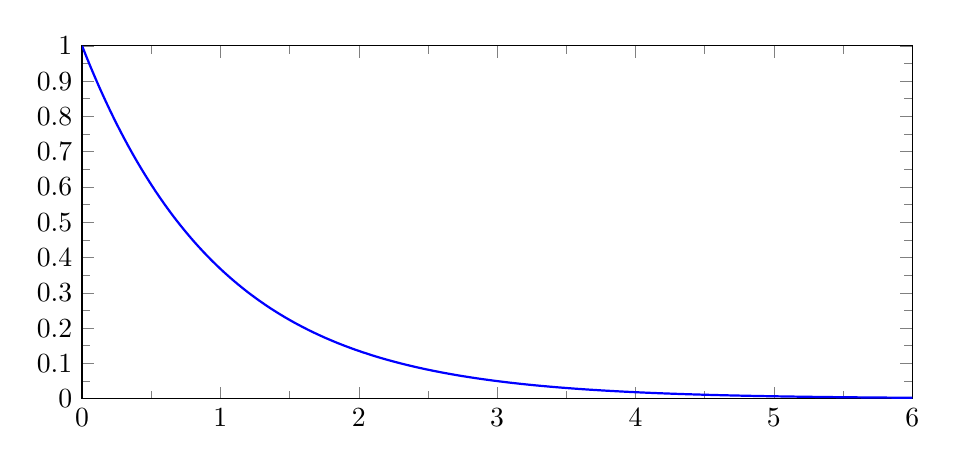
\begin{tikzpicture}
        \begin{axis}[
                xmin = 0, xmax = 6,
                ymin = 0, ymax = 1,
                xtick distance = 1,
                ytick distance = 0.1,
                minor tick num = 1,
                width = \textwidth,
                height = 0.5\textwidth]
            \addplot[
                domain = 0:6,
                samples = 200,
                smooth,
                thick,
                blue,
            ] {exp(-x))};
        \end{axis}
    \end{tikzpicture}
\end{hwproof}
\section{Notebook}

\end{document}